\documentclass[a4paper]{article}

%% Language and font encodings
\usepackage[english]{babel}
\usepackage[utf8x]{inputenc}
\usepackage[T1]{fontenc}

%% Sets page size and margins
\usepackage[a4paper,top=3cm,bottom=2cm,left=3cm,right=3cm,marginparwidth=1.75cm]{geometry}

%% Useful packages

\usepackage[fleqn]{amsmath}
\usepackage{breqn}
\usepackage{graphicx}
\usepackage[colorinlistoftodos]{todonotes}
\usepackage[colorlinks=true, allcolors=blue]{hyperref}	

\title{Adaptive Kernel Density Estimation using the Generalized Method of Moments and Compressive Kernel Selection}
\author{Shima Kamyab, Behrooz Nasihatkon, Reza Boostani}

\begin{document}
\maketitle

\begin{abstract}
We formulate the problem of varying bandwidth kernel density estimation as an optimization problem. The method estimates the density function as a linear combination of a large number of kernel functions with different bandwidths. The target function is a quadratic form obtained using the Generalized Method of Moments, plus an sparsity including $L_1$ term for adaptively choosing the best kernels. 
\end{abstract}

%\begin{Keyword} 
%\textbf{Keywords:} Generalized method of moments, Adaptive Kernel Density Estimation, Sparse Density Estimation, Sparse Mixture Models.
%\end{keyword}
\section{Introduction}
%\label{sec:intro}
\input{01_Introduction.tex}

\section{Related Works}
\label{sec:rev}
%As mentioned in introduction section, in this paper, we formulate maximum likelihood estimation as a convex optimization problem with $l_1$ penalty using Generalized Method of Moments. In this section we describe some existing similar studies as follows. 
In the field of Generalized Method of Moments for estimation we can refer to \cite{lewbel2007local} in which a local Generalized Method of Moments Estimator is proposed for non-parametrically estimation of unknown functions that are defined by conditional moment restrictions. But this research is not about the density estimate and it just finds some function having moment constraints. In \cite{gopalakrishnaneecs} a method with the ability of generating kernel density estimates with a specified degree of sparsity is developed. The proposed method uses $l_0$, negative $l_2$ and weighted $l_1$ penalties in order to explicitly bring sparsity constraint into the optimization problem of estimating density. The author's state that this method can provide sparse solutions while satisfying constraints on the quality of the estimates and therefore provides a trade-off between the sparsity and the quality of the density estimates. The objective function to be minimized in this method is as
\begin{equation}
\label{e1}
\min_a{\alpha^TQ\alpha-c^T\alpha}
\end{equation}
Where,  $\alpha$ is the vector of weights. $Q_ij=k_{\sqrt{2\sigma}}(x_i,x_j), c_i=(2/m)\sum_{j=1}^mk_{\sigma}(y_j,x_i), x_i$-s are independent realization of \emph{f} (density to be estimated) used as training data and $y_i$-s are independent realization of f used as test data. This method uses data samples in the optimization formulation, while our method uses a low dimensional representation of data in the estimation process.
In \cite{hong2013sparse} a sparse kernel density estimator using a forward constrained regression framework is proposed, within which the nonnegative and summing-to-unity constraints of the mixing weights can easily be satisfied. The main contribution of this work is to derive a recursive algorithm to select significant kernel so neat time based on the minimum integrated square error (MISE) criterion for both these lection of kernels and the estimation of mixing weights. The complexity of the proposed algorithm is in the order of the number of training data $N$, which is much lower than the order of $N^2$ offered by the best existing sparse kernel density estimators. This method adaptively fits a linear combination of (gaussian) kernels into the sample data itself. In \cite{peherstorfer2014density} an adaptive sparse-grid-based density estimation method is presented which discretizes the estimated density function on basis functions centered at grid points rather than on kernels centered at the data points. Thus, the costs of evaluating the estimated density function are independent from the number of data points. This method also uses a cross validation technique for the parameter selection. Van Kerm in \cite{van2003adaptive}, proposes an adaptive kernel density estimation using an iterative procedure: An initial (fixed bandwidth) density estimate is computed to get an idea of the density at each of the data points, and this pilot estimate is used to adapt the size of the bandwidth over the data points when computing a new kernel density estimate. In \cite{botev2010kernel} a new adaptive kernel density estimator based on linear diffusion processes is proposed which builds on existing ideas for adaptive smoothing by incorporating information from a pilot density estimate. In addition, a new plug-in bandwidth selection method is proposed that is free from the arbitrary normal reference rules used by existing methods. In \cite{gine2003l1}, the notion of an l1-norm density estimator process indexed by a class of kernels is introduced. Then a functional central limit theorem and a Glivenko–Cantelli theorem are established for this process. While assembling the necessary machinery to prove these results, a body of Poissonization techniques and restricted chaining methods is developed which is useful for studying weak convergence of general processes indexed by a class of functions. None of the theorems imposes any condition at all on the underlying Lebesgue density f. Also, somewhat unexpectedly, the distribution of the limiting Gaussian process does not depend on f. \cite{bunea2010spades} Studies sparse density estimation via $l_1$ penalization (SPADES) with the focus on estimation in high-dimensional mixture models and nonparametric adaptive density estimation. This paper shows that SPADES can recover, with high probability, the unknown components of a mixture of probability densities and that it yields minimax adaptive density estimates. These results are based on a general sparsity oracle inequality that the SPADES estimates satisfy. We offer a data driven method for the choice of the tuning parameter used in the construction of SPADES. The method uses the generalized bisection method introduced in \cite{bunea2009dimension}. The suggested procedure bypasses the need for a grid search and offers substantial computational savings. In \cite{mahapatruni2011cake} a generalization of kernel density estimation called Convex Adaptive Kernel Density Estimation (CAKE), with the aim of minimizing the $l_2$ error of an estimator also known as the integrated squared error (ISE), is presented that replaces single bandwidth selection by a convex aggregation of kernels at all scales, where the convex aggregation is allowed to vary from one training point to another.
A sparse reduced set density estimator with weighted $l_1$ penalty term (RSDE-WL1) is proposed in \cite{yang2015sparser}. By introducing the weighted $l_1$ norm of the estimated coefficients as additional penalty term, the sparse weights of density estimation are estimated, in which small weight coefficients are more likely to be driven to zero. The proposed iterative algorithm is used to solve the corresponding convex optimization problem efficiently. Some discussions about the choice of parameters and the trade-off between sparsity and accuracy are also given. In \cite{bunea2007sparse} it is shown that the penalized least squares estimator satisfies sparsity oracle inequalities, i.e., bounds in terms of the number of non-zero components of the oracle vector. This paper considers estimators of density functions f that belong to the linear span of a set of $M$ basis functions $\{f_1, \ldots, f_M\}$. Let $f_{\lambda}$  denotes the linear combinations:

\begin{equation}
\label{e2}
f_{\lambda}(x)=\sum_{j=1}^M \lambda_jf_j  \hspace{2cm} \lambda=(\lambda_1,\ldots, \lambda_M) \in R^M
\end{equation}
  
This paper defines  $\hat{\lambda}$  ¸ as a minimizer of an $l_1$-penalized criterion, that is called SPADES (SPArse Density Estimation). \par
In \cite{hong2016sparse} a new sparse kernel density estimator with tunable kernels is introduced within a forward constrained regression framework where, by the nonnegative and summing-to-unity constraints of the mixing weights can easily be satisfied. Based on the minimum integrated square error criterion, a recursive algorithm is developed to select significant kernels one at time, and the kernel width of the selected kernel is then tuned using the gradient descent algorithm. In \cite{hong2010sparse} a sparse kernel density estimator is derived based on the zero-norm constraint, in which the zero-norm of the kerne1 weights is incorporated to enhance model sparsity. The classical Parzen window estimate is adopted as the desired response for density estimation, and an approximate function of the zero-norm is used for achieving mathematical tractability and algorithmic efficiency. Under the mild condition of the positive definite design matrix, the kernel weights of the proposed density estimator based on the zero-norm approximation can be obtained using the multiplicative nonnegative quadratic programming algorithm. In \cite{krauthausen2011sparse} the estimation of conditional densities of continuous random variables from noisy samples is considered. The conditional densities are modeled as heteroscedastic Gaussian mixture densities allowing for closed-form solution of Bayesian inference with full densities. The key idea is a regularization based on the curvature of the conditional density function’s surface. The main contributions are the introduction of a superficial regularizer, the consideration of model uncertainty relative to the local data distribution by means of adaptive covariances, and an efficient distance-based estimation algorithm leading to an improved generalization quality of the estimates. The proposed algorithm is an iterative two-step optimization scheme for hyperparameters and the components’ parameters. The obtained solutions are sparse, smooth, and generalize well.
None of above studies has the convex optimization and sparsity and adaptation of bandwidth together in a convex optimization framework on a low dimensional representation of the data. The most similar work to us is \cite{hong2016sparse} which we compare our results to this method in simulation section of this paper.

\section{Our Method}
\label{sec:prop}
%We start by an example. Consider a random variable $X$ with a Gamma distribution $\Gamma(k,\theta)$  . The mean and second moments are respectively equal to $\varepsilon(X)=k\theta$  and $\varepsilon(X^2)=k(k+1)\theta^2$ . Given a set of sample points $x_1, …, x_n $, we could compute $y_1=\sum_{i=1}^nx_i/N$ and $y_2=\sum_{i=1}^n x_i^2/N$  . We can estimate the distribution parameters $k$ and $\theta$ by solving the polynomial equations:

\begin{align}
  \label{eq:poly_eq}
  k \theta  &= y_1,
  \\
  k (k-1) \theta^2 &= y_2.
\end{align}
This solution, of course, is not generally optimal in the Maximum-likelihood sense. To get a better estimation, one may think
of adding more equations. For example, by adding the third moment of $X$, we get $k (k+1) (k+2) \theta^3 = y_3 = \sum_{i=1}^n
x_i^2/N$. In this way, we obtain an overdetermined system of polynomial equations. Now, the question is how to combine these
equations such that the final solution is (close to) optimal in terms of maximum-likelihood. It is the object of this paper to
provide an answer to this question.

\subsection{The Method}
Consider a set of independent sample points $x_1, x_2,\ldots,x_N \in R ^d$ drawn from a distribution with the parametric
density function $f_\theta\colon \Omega \subseteq R^d \rightarrow R$. 
To estimate the set of parameters $\theta$ we take the following approach. 
Consider a set of
functions $k_1,k_2,\ldots, k_M$ with $k_j\colon R^d \rightarrow R$. For each function, we consider the random variables
$y_j = \sum_{i=1}^N k_j(x_i) / N$. The idea is to maximize the likelihood with respect to the variables $y_j$, rather
than the samples $x_i$. We arrange $y_j$-s in a vector $y$, that is
\begin{align}
 \label{eq:y}
  y =  \frac{1}{N} \sum_{i=1}^N k(x_i). 
\end{align}
where $k(x_i) = [k_1(x_i), \ldots, k_M(x_i)]^T$. The key observation is that $y$ is the sum of $N$ random vectors with the
same distribution, and thus, its distribution can be well approximated with a Gaussian given sufficiently many
sample points due to the \emph{Central Limit Theorem}. The mean of this distribution is
\begin{align}
  \label{eq:e}
 \mu = \varepsilon(y) = \int_\omega k(x) f_\theta(x) dx, 
\end{align}
and its covariance matrix is equal to  
\begin{align}
  \label{eq:cov}
  C = \varepsilon((y-\mu)(y-\mu)^T) = \frac{1}{N} \, \varepsilon\left(k(x)k(x)^T\right) - \frac{1}{N}\, \mu\,\mu^T.
\end{align}
Since the distribution of $y$ is approximation by a Gaussian, the maximum
likelihood solution with respect to $y$ can be approximated as
\begin{align}
  \label{eq:ml_y}
  \theta^* &= (\mu_\theta - y)^T C_\theta^{-1} (\mu_\theta - y)
\end{align}
where the subscript in $\mu_\theta$ and $C_\theta$ indicates that they are function of $\theta$. If the covariance matrix is
somehow estimated as $\hat{c}$, the above turns to a (generally nonlinear) maximum likelihood problem
\begin{align}
  \label{eq:ml_y_ls}
  \theta^* &= \underset{\theta}{\operatorname{argmin}}(\mu_\theta - y)^T \hat{c}^{-1} (\mu_\theta - y). 
\end{align}
Returning to our problem in the introduction section, \ref{eq:ml_y_ls} gives a way of (nearly) optimally solving the
overdetermined set of equations $\mu_\theta = y$. We try to choose functions $k_j$ such that $\mu_\theta$ gets a
desirable form and \ref{eq:ml_y_ls} or \ref{eq:ml_y} become a well-behaved optimization problem. 
\subsection{Linear mixture of fixed basis functions}
Now, assume that $f$ is parameterised as a linear combination of a set of basis functions $b_k$, that is
\begin{align}
  f_w(x) = \sum_{k=1}^P w_k b_k(x) = b(x)^T w,
\end{align}
where $b\colon R^d \rightarrow R^P$ is the vertical concatenation of $b_k$-s and $w = [w_1,w_2,\ldots,w_P]^T \in R^P$. In this case, the problem \eqref{eq:ml_y_ls}
turns to
\begin{align}
  \label{eq:ml2_w}
  w^* = \underset{\theta}{\operatorname{argmin}} \left(H w - \bar{y} \right)^T \hat{c}^{-1} \left(Hw - \bar{y} \right) 
\end{align}
where, 
\begin{align}
  \label{eq:H}
  H = \int_\omega k(x) b(x)^T dx \in R^{M * P}.
\end{align}
In order to lead the problem toward finding sparse w-s, we added l1 penalty to the optimization problem. Therefore, the problem will be as \eqref{eq:sparse} 
\begin{equation}
%\begin{align*}
\label{eq:sparse}
[w^*,a^*] =\underset{w,a}{\operatorname{argmin}}\{(Hw-\bar{y})^T\hat{c}^{-1}(Hw-\bar{y})+\gamma\sum_{i=1}^Pa_i \} 
s.t \hspace{3cm} a_i \geq w_i,  a_i \geq -w_i
%\end{align*}
\end{equation}
We can write \ref{eq:sparse} as a conditional quadratic programming problem:
\begin{align*}
\label{eq:quadP}
[w^*,a^*]&=\underset{w,a}{\operatorname{argmin}}\{\frac{1}{2}(w'^TA'w')+f'^Tw'\}\\
s.t  &\hspace{2cm} a_i \geq w_i,  a_i \geq -w_i \\
\mbox{where},\\
&w_{P*1}=[w_1,\ldots,w_P]^T \\
&A_{P*P}=-2H^T\hat{c}^{-1}H \\
&f_{P*1}=-2H^T\hat{c}^{-1}\bar{y} \\
&w'_{2P*1}=[w_1, w_2, ...,w_P, a_1, a_2 , ..., a_P]^T  \\ 
&A'_{(2P*2P)}=\left[{ \begin{array}{c c}  A_{P*P} & 0 \\ 0 & 0 \\  \end{array}} \right] \\ ,  &f'_{(2P*1)} =[f_{P*1}^T,1,1,...,1]^T \\ \\
\end{align*}
In (\ref{eq:H}) we need to specify basis functions $b_i$-s and $k_j$-s. We choose $k_j$-s as 10 gaussian functions with fix bandwidths. In the case of $b_i$-s, assuming that they are gaussian kernels, we adopted an adaptive scheme for selection of appropriate bandwidths for each kernel. We put gaussian kernels with different bandwidths on each sample data and consider these kernels as $b_i$-s. In the process of quadratic programming the suitable kernel for each interval will be selected. This is shown in simulation section.

%\section{Derivations}
%\label{sec:derivs}
\subsection{No Adaptive Scheme}\label{sec:noadapt}
Suppose we have a set of $N$ sample points $X = [x_1, x_2, ..., x_N]$, independently drawn from a Gaussian mixture $f_w(x) = \sum_{i = 1}^p b_i(x)w_i(x)$, which is a weighted combination of $p$ fixed Gaussian basis functions. For the first step, let's define the objective as to estimate the weights $w_{(p \times 1)} = [w_1, w_2, ..., w_p]^T$ in the $f_w$, knowing $p$ fixed basis functions $b_{(p\times 1)} = [b_1(\cdot), b_2(\cdot), ..., b_p(\cdot)]^T$.\par
The idea is to assume a set of (kernel) functions $k_{(m \times 1)} = [k_1(\cdot), k_2(\cdot),..., k_m(\cdot)]^T$ and define the new random variable $y$ as:
\begin{equation}
    y_{(m \times 1)} = 1/N \sum_{i=1}^N k(x_i)
\end{equation}
because $y$ is sum of some random variables with the same distribution, it ($y$) has a Gaussian distribution (Central limit theorem). Our new aim is then to estimate the distribution of $y$ using the maximum likelihood method. The maximum likelihood objective is to:
\begin{equation} \label{eq:prop_obj1}
    min_{w} 1/2(E(y) - y)^TC^{-1}(E(y) - y)
\end{equation}
where
\begin{align}
    E(y)_{(m \times 1)} = \int k(x)f_w(x) dx \\
    = \left[\int k_{(m \times 1)}(x)b^T_{(1 \times p)}(x)dx \right]w_{{p \times1}} \\
    =Dw
\end{align}
and $C^{-1}_{(m \times M)}$ is the covariance matrix of $y$ which we compute it empirically. For computing $C^{-1}$, we draw $N$ samples from the distribution for $T$ times and compute $T$ random variables $y$ and then compute the covariance matrix of $T$ computed $ys$. \par
 We also add a sparsity term to the objective \eqref{eq:prop_obj1} as :
 \begin{align}
     min_{w,a} \quad 1/2(Dw - y)^TC^{-1}(Dw - y) +\gamma \sum_{i = 1}^p a_i \\
     s. t. \quad a_i \geq w_i, \quad a_i \geq -w_i
 \end{align}
where, $a$ is a new variable and $\gamma_{(p \times 1)}$ is the sparsity weight vector.\par To solve this optimization as a quadratic-programming using matlab, we should write it in the form of standard form:
\begin{align}
    min_x \quad x^THx + f^Tx \\
    s. t. \quad Ax \leq b
\end{align}
Therefore, in our problem, we have:
\begin{align}
 x_{(2p \times 1)}  = \left[ \begin{array}{c} w_{(p \times 1)}\\ a_{(p \times 1)} \end{array} \right] \\
 H_{(2p \times 2p)} = \left[ \begin{array}{cc} -(D^TC^{-1}D)_{(p \times p)} & 0\\0&0\end{array} \right] \\
 f_{(2p \times 1)} = \left[ \begin{array}{c}{(2y^TC^{-1}D)^T_{(p \times 1)}}\\\gamma_{(p \times 1)} \end{array} \right]\\
A_{(2p \times 2p)} = \left[ \begin{array}{cccccccccc}1&0&...&0&-1&0&...&0\\0&1&...&0&0&-1&...&0\\&&&&&&&&&\\0&0&...&1&0&0&...&-1\\
-1&0&...&0&-1&0&...&0\\0&-1&...&0&0&-1&...&0\\&&&&&&&&&\\0&0&...&-1&0&0&...&-1\\\end{array}\right]\\
b_{(2p \times 1)}=0_{(2p \times 1)}
\end{align}
%%%%%%%%%%%%%%%%%%%%%%%%%%%%%%%%%%%%%
%\subsubsection{Primary Results Without Adaptive Scheme}
%Fig.\ref{fig:primary_res} shows the estimated density obtained by the proposed method.
%\begin{figure}[hbt!]
%\centering
%\begin{tabular}{cc}
%\includegraphics[scale = 0.5]{Figures/primary_res_no_adaptive.PNG}     & \includegraphics[scale = 0.5]{Figures/gamma.PNG} \\
%     & 
%\end{tabular}
%\caption{primary results without adaptive setup}
%\label{fig:primary_res}
%\end{figure}
%%%%%%%%%%%%%%%%%%%%%%%%%%%%%%
\subsection{Considering Adaptive Scheme}
Taking into account the adaptive scheme means that we consider different bandwidths for each basis function $b_i(\cdot)$. Therefore, by considering $q$ fixed bandwidths for each basis function $b_i(\cdot)$, we have:\par%and adding a temporal laplacian regularization term~\cite{li2015temporal} to optimization problem, we have:
\begin{align}
     min_{w,a} \quad 1/2(Dw - y)^TC^{-1}(Dw - y) +\gamma \sum_{i = 1}^{pq} a_i \\% + \beta w^TLw \\
     s. t. \quad a_i \geq w_i, \quad a_i \geq -w_i\\
     %L_{ij}(pq \times pq)= \left\{ \begin{array}{cc} 1 & |i-j|<\frac{s}{2}\\ 0& o.w.\end{array} \right\\
    B_{(pq \times 1)} =[b_{11}, b_{21} ,..., b_{p1}, ..., b_{pq}]^T\\% \left[ \begin{array}{cccc}b_{11}& b_{21} &...& b_{p1}\\ b_{12}& b_{22} &...& b_{p2}\\&&&\\b_{1q}& b_{2q} &...& b_{pq}\end{array} \right]\\
    W_{(pq \times 1)} =[w_{11}, w_{21} ,..., w_{p1}, ..., w_{pq}]^T\\% \left[ \begin{array}{cccc}w_{11}& w_{21} &...& w_{p1}\\ w_{12}& w_{22} &...& w_{p2}\\&&&\\w_{1q}& w_{2q} &...& w_{pq}\end{array} \right]\\ 
    %\sum_{k=1}^qw_{ik}=1\\
    y_{(m \times 1)} = 1/N \sum_{i = 1}^N k(x_i)\\
    f_w(x) = \sum_{i=1}^{pq} w_{i}b_{i}(x) \\%= Tr((W^TB)_{(p \times p)})\\
    E(y) = \int k(x)f_w(x) dx= \left[\int k_{(m \times 1)}(x)b^T_{(1 \times pq)}(x)dx \right]w_{pq \times 1} \\
    =Dw\\
\end{align}
Therefore, we have:
\begin{align}
 min_x \quad x^THx + f^Tx \\
 s. t. \quad Ax \leq b\\
 x_{(2pq \times 1)}  = \left[ \begin{array}{c} w_{(pq \times 1)}\\ a_{(pq \times 1)} \end{array} \right] \\
 H_{(2pq \times 2pq)} = \left[ \begin{array}{cc} -(D^TC^{-1}D)_{(pq \times pq)} & 0\\0&0\end{array} \right] \\
 f_{(2pq \times 1)} = \left[ \begin{array}{c}{(2y^TC^{-1}D)^T_{(pq \times 1)}}\\\gamma_{(pq \times 1)} \end{array} \right]\\
A_{(2pq \times 2pq)} = \left[ \begin{array}{cccccccccc}1&0&...&0&-1&0&...&0\\0&1&...&0&0&-1&...&0\\&&&&&&&&&\\0&0&...&1&0&0&...&-1\\
-1&0&...&0&-1&0&...&0\\0&-1&...&0&0&-1&...&0\\&&&&&&&&&\\0&0&...&-1&0&0&...&-1\\\end{array}\right]\\
b_{(2pq \times 1)}=0_{(2pq \times 1)}
\end{align}
%%%%%%%%%%%%%%%%%%%%%%%%%%%%%%%%%%%%%
%\subsubsection{Results Obtained using Adaptive Scheme}
%Fig.\ref{fig:primary_res} shows the estimated density obtained by the proposed method.
%\begin{figure}[hbt!]
%\centering
%\begin{tabular}{cc}
%\includegraphics[scale = 0.5]{Figures/Adaptive/lin_apx_ml_s_2_beta_0.PNG}     & \includegraphics[scale = 0.5]{Figures/Adaptive/gamma_lin_apx_ml_s_2_beta_0.PNG} \\
 %    \multicolumn{2}{c}{$\beta = 0$} \\
%\includegraphics[scale = 0.7]{Figures/Adaptive/lin_apx_ml_s_2_beta_05.PNG}     & \includegraphics[scale = 0.5]{Figures/Adaptive/gamma_lin_apx_ml_s_2_beta_05.PNG} \\
 %    \multicolumn{2}{c}{$\beta = 0.5$} \\
%\includegraphics[scale = 0.6]{Figures/Adaptive/lin_apx_ml_s_2_beta_1.PNG} %    & \includegraphics[scale = 0.6]{Figures/Adaptive/gamma_lin_apx_ml_s_2_beta_1.PNG} \\
 %    \multicolumn{2}{c}{$\beta = 1$} 
%\end{tabular}
%\caption{primary results with adaptive scheme }
%\label{fig:primary_res}
%\end{figure}
%%%%%%%%%%%%%%%%%%%%%%%%%%%%%%
\section{SPADES~\cite{bunea2010spades} Method}
In this section we demonstrate the method proposed in~\cite{bunea2010spades}, which is a similar work to us. Suppose we have a set of $N$ sample points $X = [x_1, x_2, ..., x_N]$, independently drawn from a Gaussian mixture $f_w(x) = \sum_{i = 1}^{pq} b_i(x)w_i(x)$, which is a weighted combination of $p$ fixed Gaussian basis functions. For the first step, let's define the objective as to estimate the weights $w_{(pq \times 1)} = [w_1, w_2, ..., w_{pq}]^T$ in the $f_w$, knowing $pq$ fixed basis functions $b_{(pq\times 1)} = [b_1(\cdot), b_2(\cdot), ..., b_{pq}(\cdot)]^T$.\par, the objective in~\cite{bunea2010spades} is:
\begin{equation}
\begin{aligned}
    \min_{w, a} \left\{ -\frac{2}{N} \sum_{i=1}^N f_w(x_i) + ||f_w||^2 + \gamma\sum_{i=1}^{pq} a_i \right\}\\
    s. t. \quad a_i > w_i, a_i \geq -w_i
\end{aligned}   
\end{equation}
with
\begin{equation}
\begin{split}
||f_w(x)||^2 = \int (f_w(x))^2 dx = \int (w_jb_j(x))dx \\
= \int \sum_{j=1}^p \sum_{k=1}^p w_j w_kb_j(x) b_k(x)dx \\
= \sum_{j=1}^p \sum_{k=1}^p w_j w_k \int b_j(x) b_k(x) dx \\
= w^TCw
\end{split}
\end{equation}
and
\begin{equation}
c_{jk} = \int b_j(x) b_k(x) dx
\end{equation}
Using Matlab quadratic programming, we have:
\begin{equation}
    \begin{aligned}
    \min_x \quad x^THx + f^Tx\\
    s. t. \quad Ax \leq b \\
    x = \left[ \begin{array}{c} w_{pq \times 1}\\ a_{pq \times 1} \end{array} \right],\\
    H_{2pq \times 2pq} =  \left[ \begin{array}{cc} C_{pq \times pq} & 0\\0 & 0 \end{array}  \right], \\
    f_{2pq \times 1}=\left[ \begin{array}{c} -\frac{2}{N}\sum_{i=1}^N b_{pq \times 1}(x_i)\\\gamma_{pq \times 1}\end{array} \right], \\
    A_{(2pq \times 2pq)} = \left[ \begin{array}{cccccccccc}1&0&...&0&-1&0&...&0\\0&1&...&0&0&-1&...&0\\&&&&&&&&&\\0&0&...&1&0&0&...&-1\\
-1&0&...&0&-1&0&...&0\\0&-1&...&0&0&-1&...&0\\&&&&&&&&&\\0&0&...&-1&0&0&...&-1\\\end{array}\right]\\
b_{(2pq \times 1)}=0_{(2pq \times 1)}
    \end{aligned}
\end{equation}


\section{Simulation Study}
\label{sec:sim}
Figure~\ref{fig:cmp_res} shows the results obtained by the proposed AKDE compared to SPADES~\cite{bunea2010spades} method. We set $N=500, \gamma = 7, pq = 1500$ for this experiment.
\begin{figure}[hbt!]
\vspace{-2cm}
    \hspace{-2cm}
    \begin{tabular}{ccc}
    $f_0$& $f_1$ & $f_2$\\
         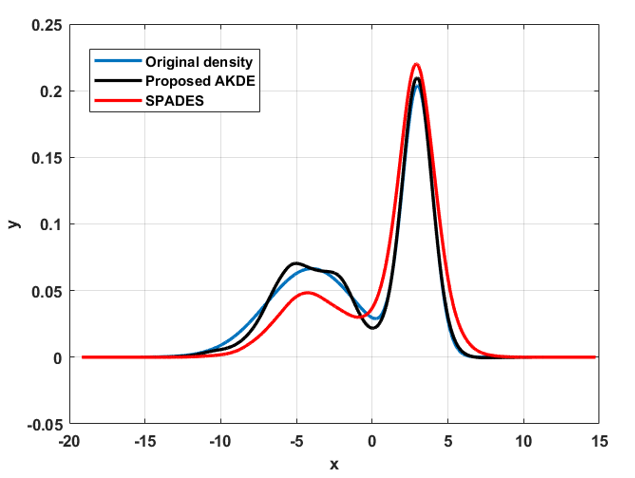
\includegraphics[scale = 0.42]{Figures/Adaptive/cmp_reults/0.PNG}&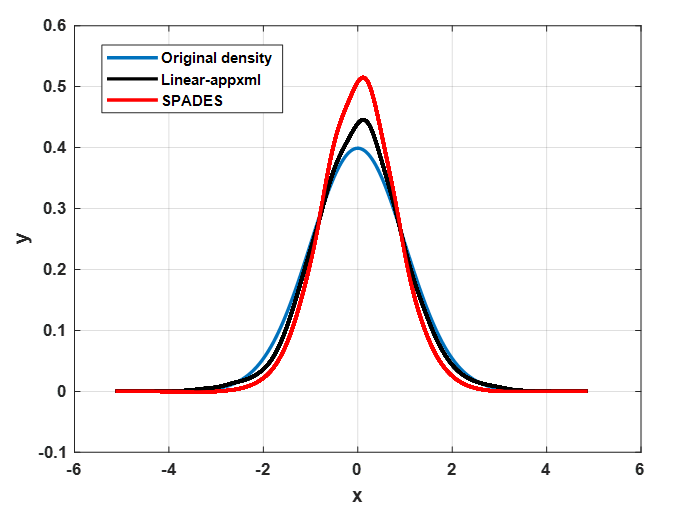
\includegraphics[scale = 0.38]{Figures/Adaptive/cmp_reults/1.PNG} &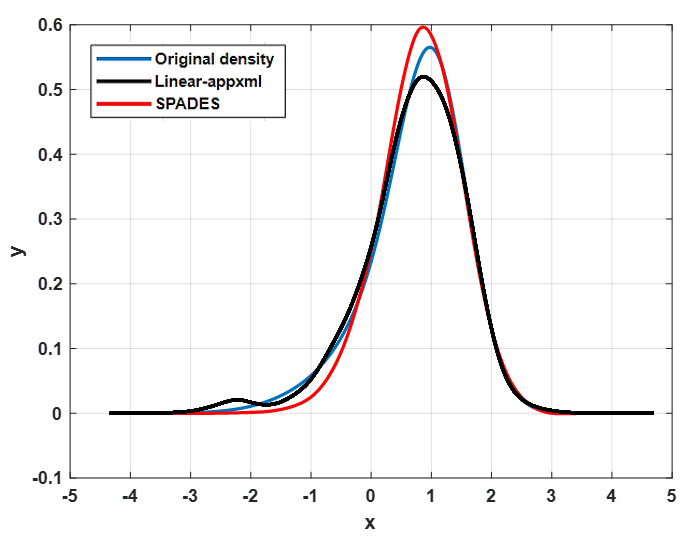
\includegraphics[scale = 0.36]{Figures/Adaptive/cmp_reults/2.PNG} \\
         \begin{tabular}{c}Averge $MSE_{Proposed} = 5.1808e-04$ \\ Average $MSE_{SPADES} =4.1e-03$\end{tabular}&\begin{tabular}{c}Averge $MSE_{Proposed} = 2.7e-03$\\ $Average MSE_{SPADES} =2.3e-02$\end{tabular}&\begin{tabular}{c}Averge $MSE_{Proposed} = 4.5e-03$ \\ Average $MSE_{SPADES} =2.2e-02$\end{tabular}\\
         $f_3$& $f_4$ & $f_5$\\
          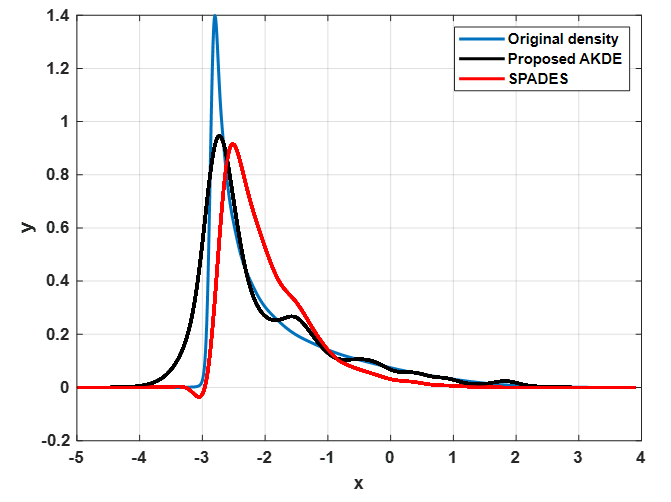
\includegraphics[scale = 0.38]{Figures/Adaptive/cmp_reults/3.PNG}&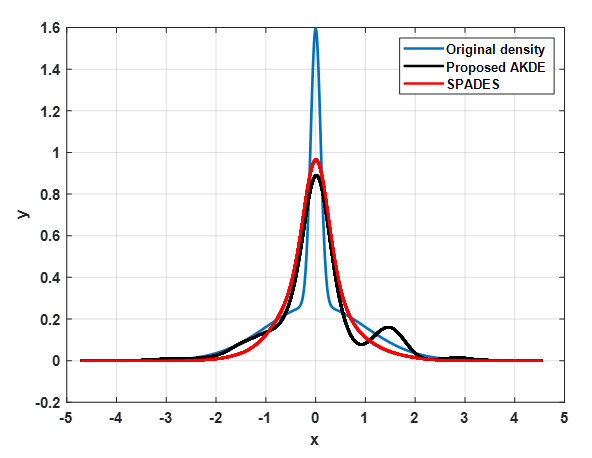
\includegraphics[scale = 0.43]{Figures/Adaptive/cmp_reults/4.PNG}&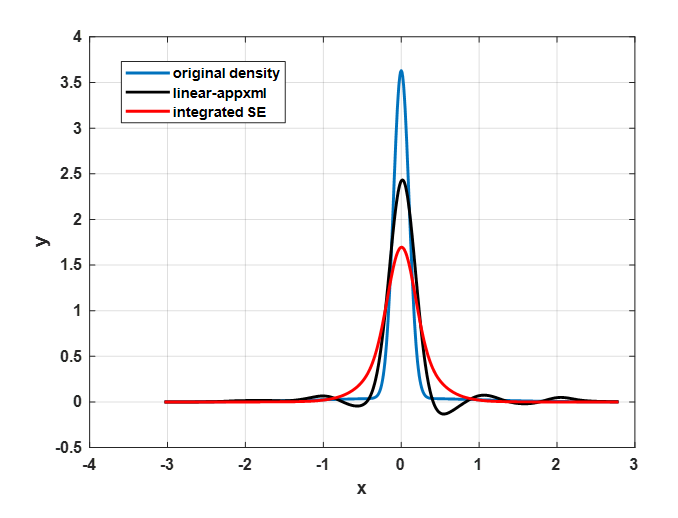
\includegraphics[scale = 0.4]{Figures/Adaptive/cmp_reults/5.PNG} \\
          \begin{tabular}{c}Averge $MSE_{Proposed} = 6.0e-02$ \\ Average $MSE_{SPADES} =3.4e-02$\end{tabular}&\begin{tabular}{c}Averge $MSE_{Proposed} = 1.6e-01$ \\ Average $MSE_{SPADES} =5.3e-02$\end{tabular}&\begin{tabular}{c}Averge $MSE_{Proposed} = 3.1$ \\ Average $MSE_{SPADES} =2.4e-01$\end{tabular}\\
          $f_6$& $f_7$ & $f_8$\\
           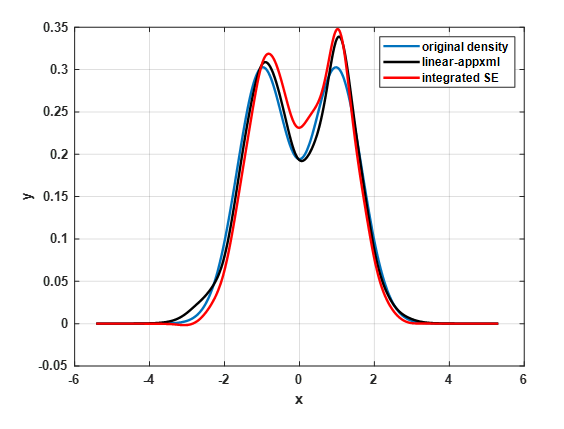
\includegraphics[scale = 0.45]{Figures/Adaptive/cmp_reults/6.PNG}&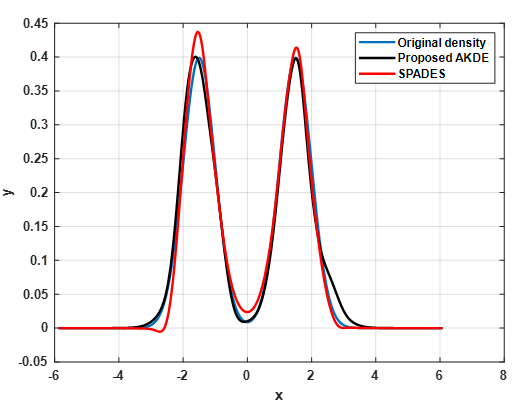
\includegraphics[scale = 0.45]{Figures/Adaptive/cmp_reults/7.PNG}&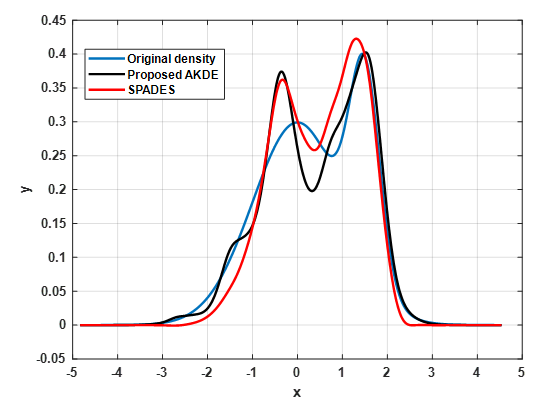
\includegraphics[scale = 0.45]{Figures/Adaptive/cmp_reults/8.PNG} \\
          \begin{tabular}{c}Averge $MSE_{Proposed} = 3.1e-03$ \\ Average $MSE_{SPADES} =1.9e-02$\end{tabular}&\begin{tabular}{c}Averge $MSE_{Proposed} = 3.0e-03$ \\ Average $MSE_{SPADES} =2.1e-02$\end{tabular}&\begin{tabular}{c}Averge $MSE_{Proposed} = 3.6e-03$ \\ Average $MSE_{SPADES} =1.8e-02$\end{tabular}\\
          $f_{9}$& $f_{10}$ & $f_{11}$\\
          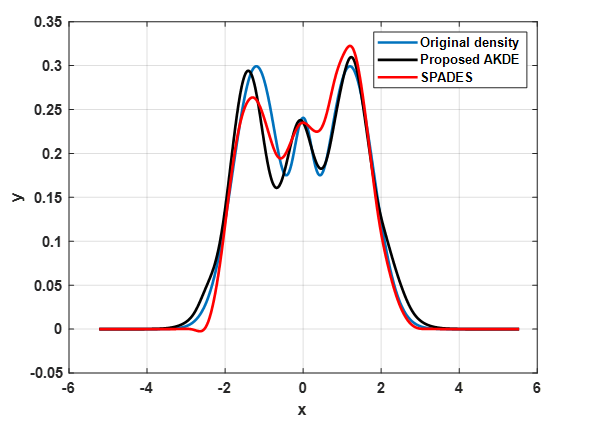
\includegraphics[scale = 0.46]{Figures/Adaptive/cmp_reults/9.PNG}&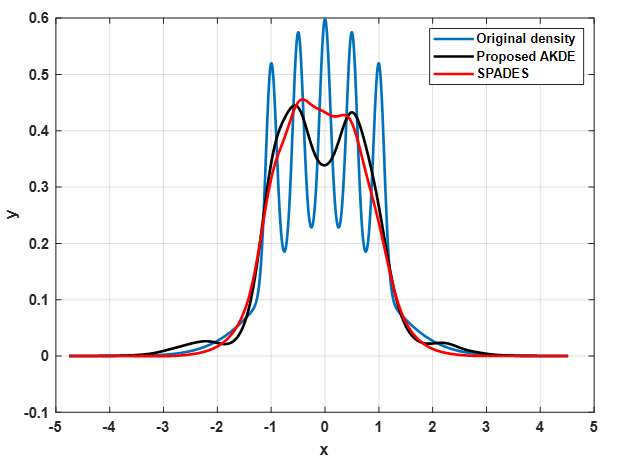
\includegraphics[scale = 0.45]{Figures/Adaptive/cmp_reults/10.PNG}&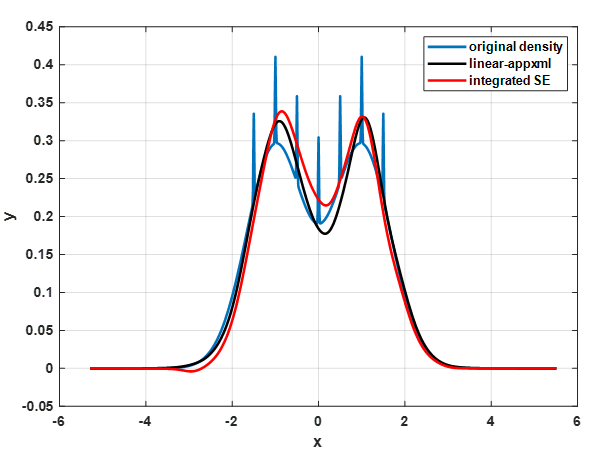
\includegraphics[scale = 0.45]{Figures/Adaptive/cmp_reults/11.PNG} \\
          \begin{tabular}{c}Averge $MSE_{Proposed} = 3.0e-03$ \\ Average $MSE_{SPADES} =1.3e-02$\end{tabular}&\begin{tabular}{c}Averge $MSE_{Proposed} = 2.0e-02$ \\ Average $MSE_{SPADES} =1.6e-02$\end{tabular}&\begin{tabular}{c}Averge $MSE_{Proposed} = 2.6e-03$ \\ Average $MSE_{SPADES} =1.2e-02$\end{tabular}\\
          $f_{12}$& $f_{13}$ & $f_{14}$\\
          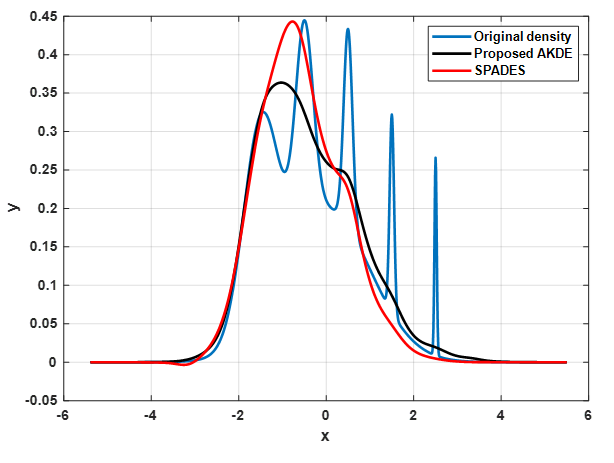
\includegraphics[scale = 0.46]{Figures/Adaptive/cmp_reults/12.PNG}&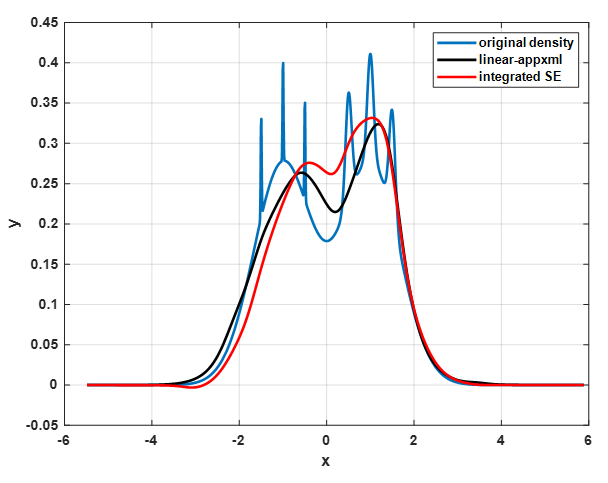
\includegraphics[scale = 0.45]{Figures/Adaptive/cmp_reults/13.PNG}&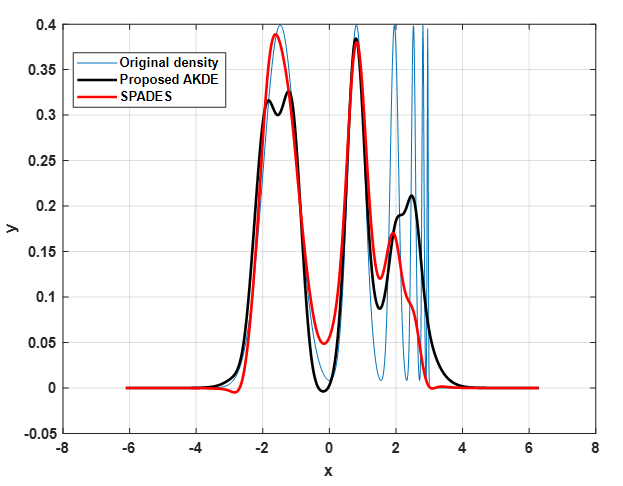
\includegraphics[scale = 0.45]{Figures/Adaptive/cmp_reults/14.PNG} \\
          \begin{tabular}{c}Averge $MSE_{Proposed} = 8.4e-03$ \\ Average $MSE_{SPADES} =1.6e-02$\end{tabular}&\begin{tabular}{c}Averge $MSE_{Proposed} = 4.1e-03$ \\ Average $MSE_{SPADES} =1.5e-02$\end{tabular}&\begin{tabular}{c}Averge $MSE_{Proposed} = 2.4e-02$ \\ Average $MSE_{SPADES} =2.0e-02$\end{tabular}\\
    \end{tabular}
    \caption{Results obtained by proposed method (marked as black) compared to  SPADES~\cite{bunea2010spades} (marked as red) method for nonparametric adaptive kernel density estimation.}
    \label{fig:cmp_res}
\end{figure}
%%%%%%%%%%%%%%%%%%%%%%%%%%%%%%%%%%%%%%%%%%%%%%%
Figure~\ref{fig:N} shows average MSE over 10 runs for proposed AKDE and spades methods. We set $pq = 600, \gamma = 7$ for this experiment.
\begin{figure}
    \hspace{-1cm}
    \begin{tabular}{ccc}
    $f_{0}$& $f_{1}$ & $f_{2}$\\
        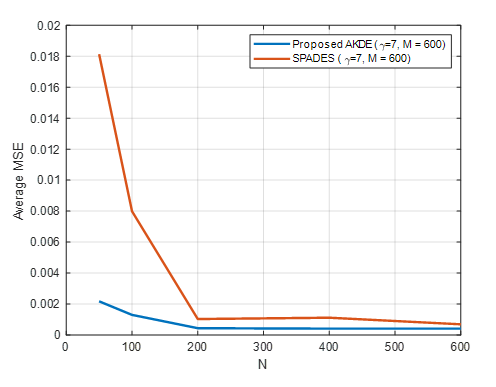
\includegraphics[scale = 0.5]{Figures/Adaptive/N/0.PNG} & 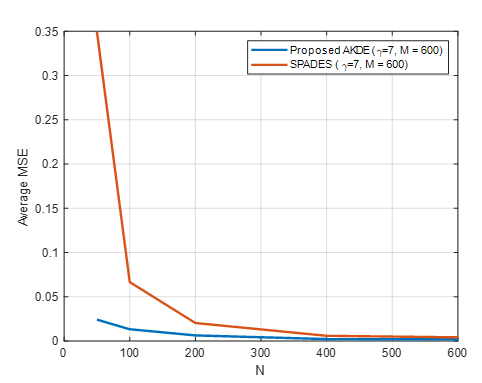
\includegraphics[scale = 0.5]{Figures/Adaptive/N/1.PNG} & 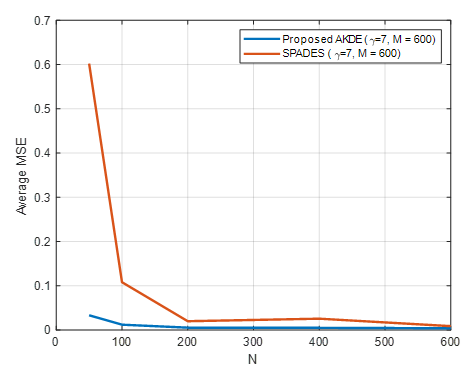
\includegraphics[scale = 0.5]{Figures/Adaptive/N/2.PNG}   \\
    $f_{3}$& $f_{4}$ & $f_{5}$\\
        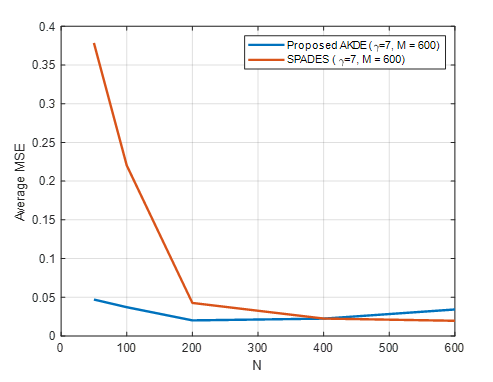
\includegraphics[scale = 0.5]{Figures/Adaptive/N/3.PNG} & 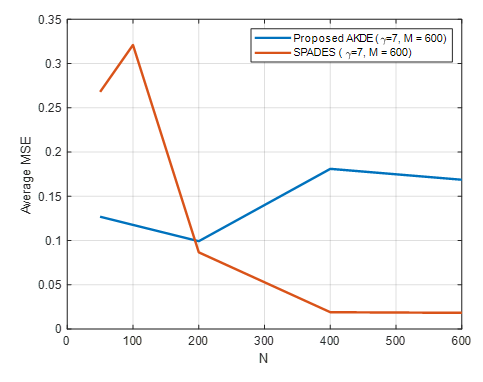
\includegraphics[scale = 0.5]{Figures/Adaptive/N/4.PNG} & 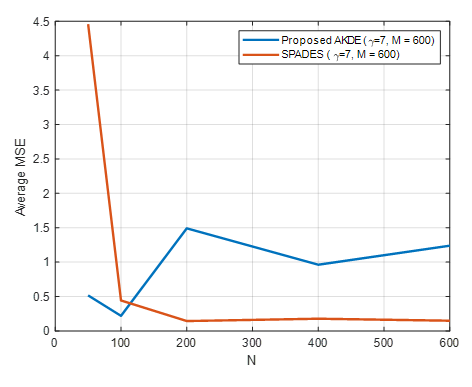
\includegraphics[scale = 0.5]{Figures/Adaptive/N/5.PNG}   \\
    $f_{6}$& $f_{7}$ & $f_{8}$\\
        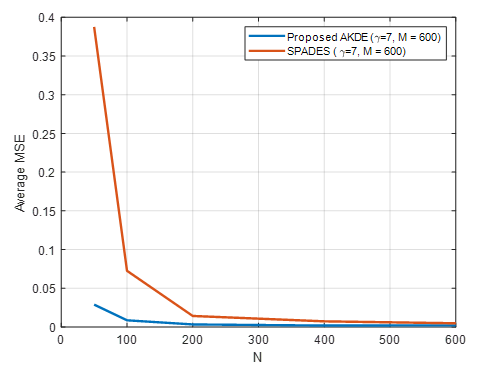
\includegraphics[scale = 0.5]{Figures/Adaptive/N/6.PNG} & 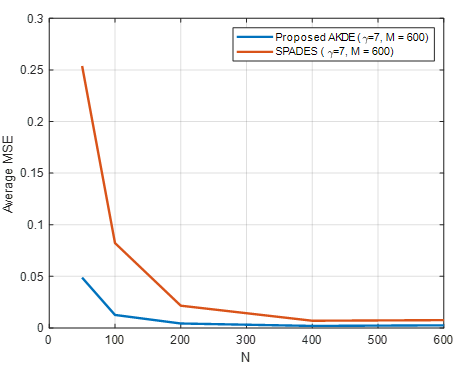
\includegraphics[scale = 0.5]{Figures/Adaptive/N/7.PNG} & 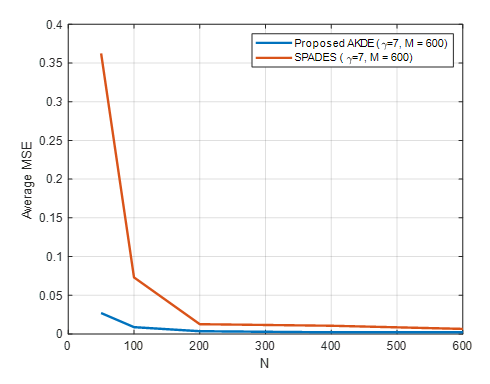
\includegraphics[scale = 0.5]{Figures/Adaptive/N/8.PNG}   \\
    $f_{9}$& $f_{10}$ & $f_{11}$\\
        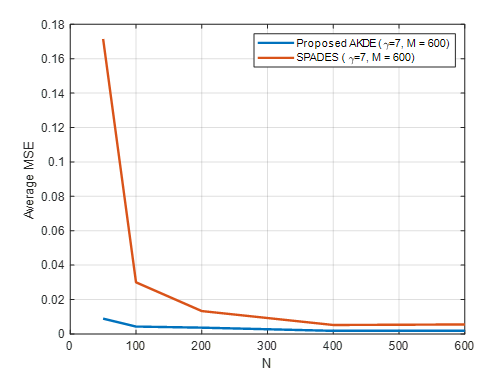
\includegraphics[scale = 0.5]{Figures/Adaptive/N/9.PNG} & 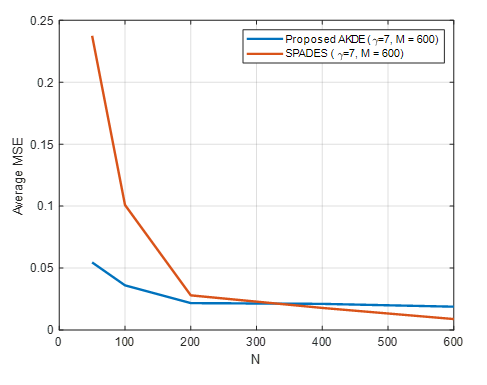
\includegraphics[scale = 0.5]{Figures/Adaptive/N/10.PNG} & 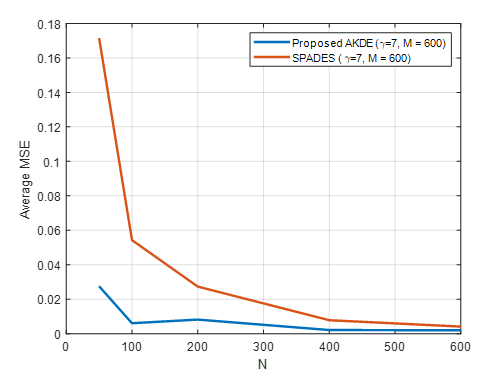
\includegraphics[scale = 0.5]{Figures/Adaptive/N/11.PNG}   \\
    $f_{12}$& $f_{13}$ & $f_{14}$\\
        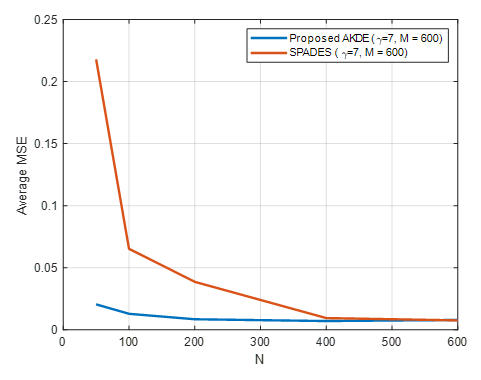
\includegraphics[scale = 0.5]{Figures/Adaptive/N/12.PNG} & 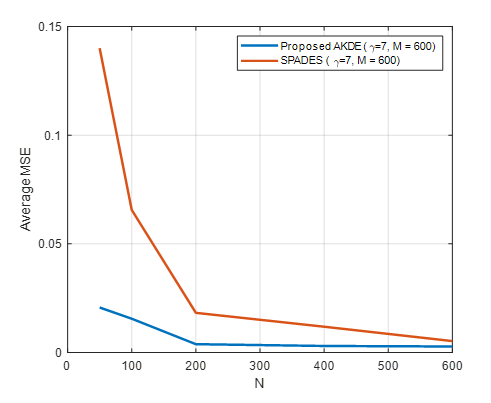
\includegraphics[scale = 0.5]{Figures/Adaptive/N/13.PNG} & 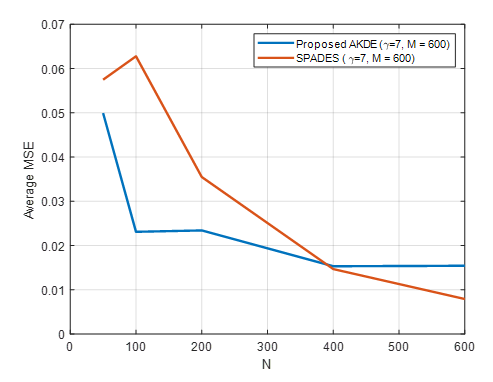
\includegraphics[scale = 0.5]{Figures/Adaptive/N/14.PNG}   \\
         
    \end{tabular}
    
    \caption{Diagram of MSE v.s. number of samples drawn from each density for 15 one dimensional densities.}
    \label{fig:N}
\end{figure}

\section{Remarks and Future work}
\label{sec:numerical}
In practice, when a large number of highly correlated $k_j$-s are used, due to computational limitations, the matrix $C$ is
usually rank deficient or ill-conditioned. In such cases the inverse matrix $C^{-1}$ cannot be computed. Consider the
eigenvalue decomposition of the symmetric positive semi-definite matrix $C$.
%\begin{align*}
%\label{eq:svd_C}
% C =V \Lambda V^T = [V_1  V_2] \Lambda  [V_1 V_2]^T 
%\end{align*}
where $V$ is the square matrix of eigenvectors, $\Lambda$ is the diagonal matrix of eigenvalues, and $[V_1 V_2]$
represents the splitting of $V$ such that $V_2$ contains the eigenvectors corresponding to the zero eigenvalues. If the
vector $e$ is distributed according to the covariance matrix $C$, then $e$ has to lie on the subspace spanned by the columns
of $V_1$. Alternatively, $V_2^T e$ vanishes for any realization of $e$.  Therefore, we need to add the constraint $V_2^T
e = V_2^T(Hw - b ) = 0$ In this case, the optimization problem \ref{eq:ml2_w} can be modified as 
%\begin{align}
%\label{eq:ml2_w_rank_def}
%w^* &= \underset{\theta}{\operatorname{argmin}} (H w - \bar{y})^T c^\dagger (Hw - \bar{y} ) 
%\text{subject to}\\
%& V_2^TH  w = V_2^T b \\
%&a_i \geq w_i,  a_i \geq -w_i
%\end{align}
where $C^{\dagger}$ is the pseudo-inverse. The above turns into a quadratic programming problem if the linear constraint $V_2^THw =
V_2^T b$ is feasible.
\bibliographystyle{acm}
\bibliography{references}
\end{document}